\section{Introduction}
The real life object chosen for this project is a perfume made of golden aluminium bottle as can be seen in figure \ref{fig:ref}.

\begin{figure}[htpb]
  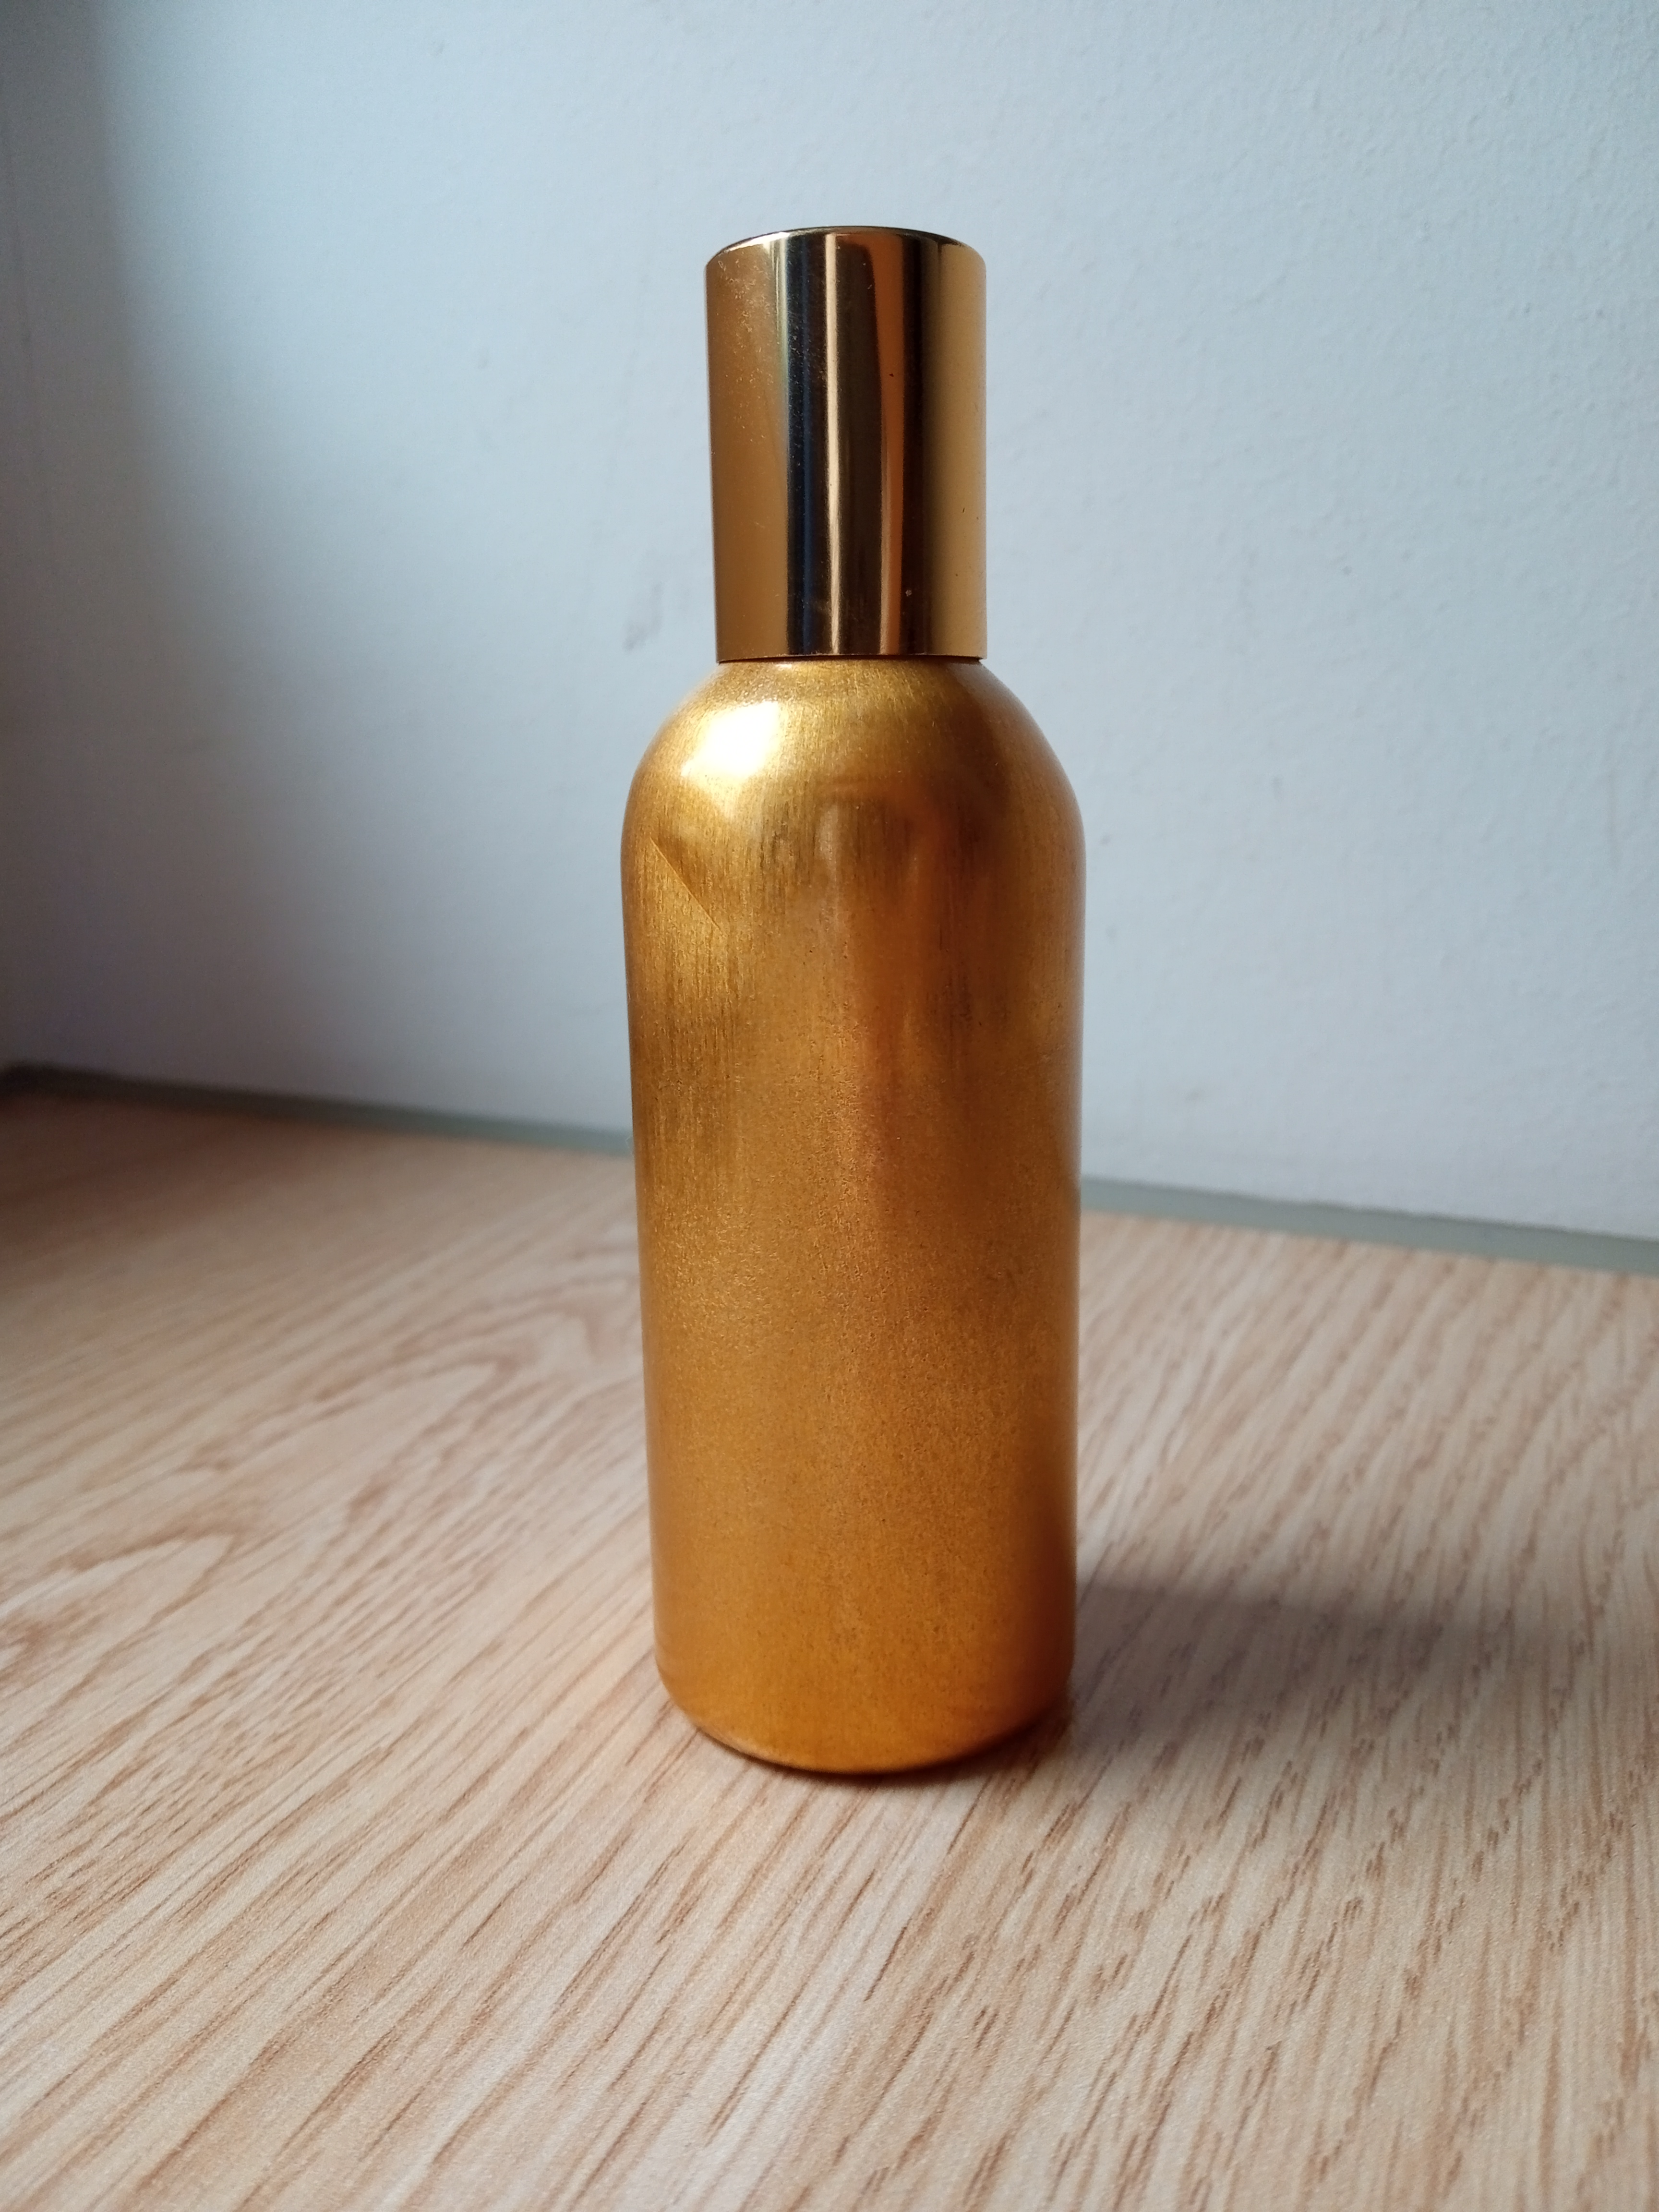
\includegraphics[width=3cm]{imgs/ref.jpg}
  \caption{Reference image}
  \label{fig:ref}
\end{figure}

This object is chosen because it can be constructed with simple primitives and there are some dirt and scratches which would be interesting to reproduce. Different parts of the object from various angles were taken for reference, which will be used for different steps in the process.
%%%%%% //DESCRIBE THE OBJECT/REFERENCE IMAGE
This report will describe the steps to produce a rendered scene containing the object.

% About 200 words for each step + 100 for intro, conclusion